\chapter{Week 10 -- Online Parameter Estimation}


\section{Abstract}
This report presents an implementation of two methods for online estimation of battery model parameters. Recursive Least Squares (RLS) take a discrete-time transfer function and search for values of its coefficients. An Extended Kalman Filter (EKF) on the other hand considers the system in the state-space augmented by auxiliary states representing the -- possibly time-varying -- system parameters and estimates those. Both methods were derived for the battery equivalent circuit model with a single RC element and tested using a recording of a dynamic discharge profile.


\section{Recursive Least Squares}
\label{sec:10-rls}

For simplicity, consider the RLS algorithm for a simple ARX model, i.e. a general discrete-time transfer function in the time-domain delay operator $d$
\begin{equation}
    G(d) = \frac{Y(d)}{U(d)} = \frac{b_0 + b_1d + \dots + b_{n_b}d^{n_b}}{1 + a_1d + \dots + a_{n_a}d^{n_a}} = \frac{\sum_{i=0}^{n_b} b_i d^i}{\sum_{i=0}^{n_a} a_i d^i},
\end{equation}
usually normalized to unity $a_0$, i.e. the coefficient belonging to $y(k)$ in the corresponding difference equation
\begin{equation}
    y(k) + \sum_{i=1}^{n_a} a_i y(k-i) = \sum_{i=0}^{n_b} b_i u(k-i) + e(k)
    \label{eq:10-difference}
\end{equation}
relating past samples of the input $u$ and output $y$ up to the discrete time $k$. The variable $e(k)$ encapsulates stochastic phenomena such as noise, as well as unmodelled system dynamics.

The most recent output $y(k)$ can be predicted from \eqref{eq:10-difference} using past inputs and outputs and system parameters $\theta$ as
\begin{equation}
        \hat{y}(k) = - \sum_{i=1}^{n_a} a_i y(k-i) + \sum_{i=0}^{n_b} b_i u(k-i) ,
\end{equation}
that can be seen as a dot product
\begin{equation}
        \hat{y}(k) = \varphi^T(k) \theta(k)
        \label{eq:10-pred}
\end{equation}
of the regressor vector 
\begin{equation}
    \varphi(k) = \begin{bmatrix} -y(k-1) &-y(k-2) &\dots & -y(k-n_a) & u(k) & u(k-1) &\dots& u(k-n_b) \end{bmatrix}^T
\end{equation}
containing past inputs and outputs and the vector of parameters
\begin{equation}
    \theta(k) = \begin{bmatrix} a_1 & a_2 & \dots & a_{n_a} & b_0 & b_1 & \dots & b_{n_b} \end{bmatrix}^T.
\end{equation}

At each iteration $k$ of the RLS algorithm, the actual measured output $y(k)$ is compared with the prediction $\hat{y}(k)$ from \eqref{eq:10-pred} to find an error $e(k)$. Then the Kalman gain $K$ is calculated using the current estimate covariance matrix $\mathbf{P}$ and finally both the estimated system parameters $\hat{\theta}$ as well as the covariance matrix $\mathbf{P}$ are updated using $K$ and $e$. The algorithm can be extended by a real forgetting factor $\lambda \in \left[0, 1\right]$ used to artificially inflate the covariance matrix $\mathbf{P}$ to facilitate tracking of time-varying parameters.

The algorithm can be generalized and applied far beyond the limitation of linear ARX model. To use the RLS algorithm for any general problem, one needs to
\begin{enumerate}
    \item express the prediction task using an equation linear-in-parameters ,
    \item determine what expressions are to be estimated and belong to the parameter vector $\theta$
    \item determine what expressions are known  and belong to the regressor $\varphi$,
    \item find the (generally non-linear) mapping between parameters $\theta$ and physically meaningful parameters useful to the application.
\end{enumerate}

\subsection{RLS for battery parameters}

The continuous-time 1 RC equivalent circuit model reads
\begin{equation}
    \Ubat = \OCV - i \,R_0 - \underbrace{i \frac{R_1}{C_1  \,R_1\,  s+1}}_{U_1},
    \label{eq:10-ecm}
\end{equation}
where $i$ is the flowing current, $\Ubat$ is the measured terminal voltage, $\OCV$ is the cell's open-circuit voltage, $R_j$, $C_j$ are parameters of the model and $s$ is the Laplace transform operator. By relabeling $E = \Ubat - \OCV$, \eqref{eq:10-ecm} can be rewritten as a transfer function 
\begin{equation}
    G_\text{cont}(s) = -R_0 -\frac{R_1 }{C_1 \,R_1 \,s+1}
    \label{eq:10-tf}
\end{equation}
from the flowing current $i$ to the voltage drop $E$. The Tustin (bilinear) discretization of $G_\text{cont}(d)$ with step $T$ gives
\begin{equation}
    G(d) = \frac{{\left(R_0 \,T+R_1 \,T-2\,C_1 \,R_0 \,R_1 \right)}\,d+R_0 \,T+R_1 \,T+2\,C_1 \,R_0 \,R_1 }{{\left(2\,C_1 \,R_1 -T\right)}\,d-T-2\,C_1 \,R_1 }.
    \label{eq:10-G}
\end{equation}
Coparing \eqref{eq:10-G} to a general first-order discrete-time transfer function
\begin{equation}
    \frac{b_1 d + b_0}{a_1 d + 1}
\end{equation}
yields substitutions
\begin{align}
a_1 &=\frac{T-2\,C_1 \,R_1 }{T+2\,C_1 \,R_1 },\\
\label{eq:10-a1}
b_1 &=-\frac{R_0 \,T+R_1 \,T-2\,C_1 \,R_0 \,R_1 }{T+2\,C_1 \,R_1 },\\
b_0 &=-\frac{R_0 \,T+R_1 \,T+2\,C_1 \,R_0 \,R_1 }{T+2\,C_1 \,R_1 }.
\label{eq:10-b0}
\end{align}

Using the discretized transfer function $G(d)$, \eqref{eq:10-ecm} can be rewritten in several steps
\begin{align}
    \Ubat - \OCV &= i G(d), \\
    (\Ubat - \OCV)(a_1 d + 1) &=  i (b_1 d + b_0), \\
    \Ubat + \Ubat a_1 d - \OCV(a_1 d + 1) &=  i (b_1 d + b_0), \\
     \Ubat &= \OCV (a_1 d + 1) - \Ubat a_1 d + i (b_1 d + b_0).
     \label{eq:10-last}
\end{align}
Finally, assuming that the $\Delta \OCV$ is negligible on each sampling interval and therefore $\OCV(k) \approx \OCV(k-1)$, \eqref{eq:10-last} can be converted from the $d$-operator domain to index shifts
\begin{equation}
    \Ubat(k) = (a_1 + 1) \OCV - a_1 \Ubat(k-1) + b_0 i(k) + b_1 i(k-1).
    \label{eq:10-final}
\end{equation}
Equivalently in the short vector notation
\begin{equation}
    \Ubat(k) = \varphi^T(k) \theta,
\end{equation}
where
\begin{align}
    \theta &= \begin{bmatrix} (a_1 + 1) \OCV & a_1 & b_0 & b_1\end{bmatrix}^T, \label{eq:10-theta} \\ 
    \varphi(k) &= \begin{bmatrix} 1 & -\Ubat(k-1) & i(k) & i(k-1)\end{bmatrix}^T.
    \label{eq:10-varphi}
\end{align}

The problem at hand was successfully described using an equation \eqref{eq:10-final} that is linear in parameters $\theta$ and hence can be subject to RLS. Equations \eqref{eq:10-theta} and \eqref{eq:10-varphi} describe the role of individual variables ($\theta$ are estimated) and
equations \eqref{eq:10-a1} through \eqref{eq:10-b0} describe the nonlinear mappings from physically meaningful battery parameters to elements of $\theta$ with the inverse mapping given by
\begin{align}
R_0 &= \frac{b_0 -b_1 }{a_1 -1},\\
R_1 &= \frac{2\,{\left(b_1 -a_1 \,b_0 \right)}}{{a_1 }^2 -1}, \\
C_1 &= -\frac{T\,{a_1 }^2 -2\,T\,a_1 +T}{4\,{\left(b_1 -a_1 \,b_0 \right)}}.
\end{align}

Performance of the estimation algorithm is presented in Section \ref{sec:10-results}.

\section{Extended Kalman Filter}
\label{sec:10-ekf}

The EKF was discussed multiple times in previous reports, mainly as a great tool for SoC estimation. This time, it is used to estimate states of a state-space model augmented with model parameters. 
The 1 RC ECM from \eqref{eq:10-ecm} can be rewritten as a state-space
\begin{align}
    \dot{U_1} = - \frac{1}{R_1 C_1} U_1 + \frac{1}{C_1} i \\
    \Ubat = \OCV - i R_0 - U_1
    \label{eq:10-ss}
\end{align}
with input $i$, output $\Ubat$ and state $U_1$ (the polarization voltage). To estimate some model parameter $M$, it must be added to the list of system states. Without any apriori knowledge of parameter evolution, $\dot{M} = 0$ is assumed such that the parameter evolution is driven only by a random walk of the process noise.
Two distinct cell state-space representations based on the 1 RC equivalent circuit model were implemented and tested -- the reference model "Hongwen" with six states from \cite{hongwen} and my own manually derived model "Michal" with five states. Both models have the flowing current $i$ as input $u$ and the terminal voltage $\Ubat$ as output $y$.

\subsection{Hongwen model}
\label{sec:10-ekf-hongwen}
The Hongwen model considers six states
\begin{equation}
    x = \begin{bmatrix}
        \OCV & \Ubat & U_1  & \frac{1}{C_1} & \frac{1}{R_1} & R_0
    \end{bmatrix}^T
\end{equation}
with state equations
\begin{equation}
\begin{aligned}
    \dot{x_1} &= 0, \\
    \dot{x_2} &= x_1 x_4 x_5 - x_2x_4x_5 - (x_4 x_5 x_6 + x_4)u - x_6 \dot{u}, \\
    \dot{x_3} &= x_4 u - x_3 x_4 x_5, \\
    \dot{x_4} &= 0, \\
    \dot{x_5} &= 0, \\
    \dot{x_6} &= 0. \\
\end{aligned}
\end{equation}
This model includes the terminal voltage $\Ubat$ as state $x_2$, making the output equation trivial
\begin{equation}
    y = x_2.
\end{equation}
This model is quite complex and requires a non-standard addition of $\dot{u}$ (the derivative of input) that may introduce complications of its own.

\subsection{Michal model}
\label{sec:10-ekf-michal}
The Michal model eliminates the terminal voltage $\Ubat$ and considers only five states
\begin{equation}
    x = \begin{bmatrix}
        \OCV & U_1  & \frac{1}{C_1} & \frac{1}{R_1} & R_0,
    \end{bmatrix}^T
\end{equation}
with state equations
\begin{equation}
\begin{aligned}
    \dot{x_1} &= 0, \\
    \dot{x_2} &= x_3 u - x_2 x_3 x_4, \\
    \dot{x_3} &= 0, \\
    \dot{x_4} &= 0, \\
    \dot{x_5} &= 0 \\
\end{aligned}
\end{equation}
and a non-linear output equation
\begin{equation}
    y = x_1 - x_2 - u x_5.
\end{equation}
This model has fewer states, does not require the numeric differentiation of input $u$ and is generally much simpler than the Hongwen model. Results of online parameter estimation with both models are presented in Section \ref{sec:10-results}.

\clearpage
\section{Estimation results}
\label{sec:10-results}

All three methods (RLS estimation from Section \ref{sec:10-rls}, EKF for Hongwen model from Section \ref{sec:10-ekf-hongwen} and EKF for Michal model from \ref{sec:10-ekf-michal}) were compared using waveforms from a dynamic discharge profile. The achieved prediction error is shown in Fig. \ref{fig:10-pred}; Fig. \ref{fig:10-voltages} shows predictions throughout several DDP cycles whereas Fig. \ref{fig:10-pred-error} focuses on one DDP period. Low prediction error less than 10 mV confirms good convergence of model parameters to the behavior of the actual battery, although there is certainly some room for improvement (e.g. by introducing a second RC element).

\begin{figure}[hbp]
    \centering
\begin{subfigure}{0.49\textwidth}
    \centering
    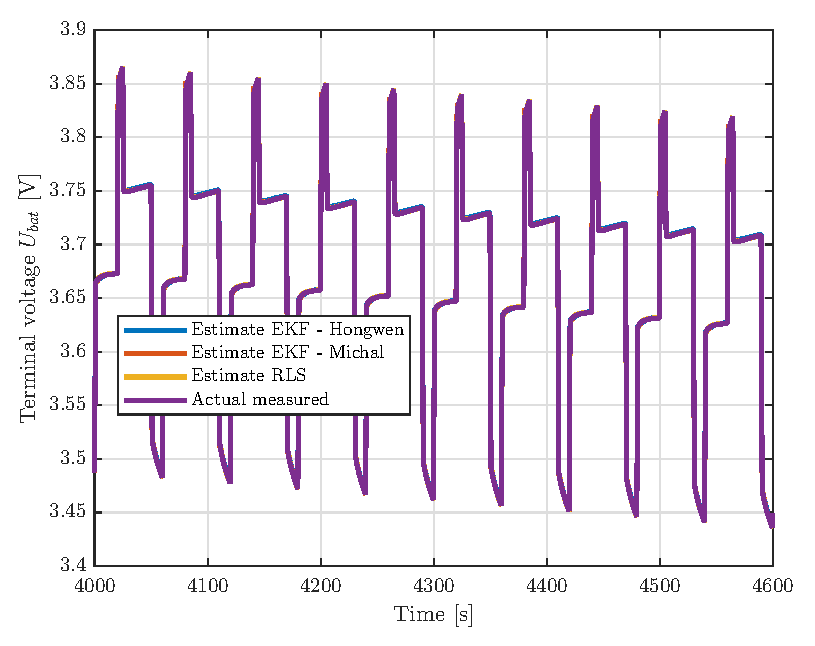
\includegraphics[width=\textwidth]{figures/10/voltages.eps}
    \caption{Over several DDP cycles.}
    \label{fig:10-voltages}
    \end{subfigure}
    \hfill
    \begin{subfigure}{0.49\textwidth}
    \centering
    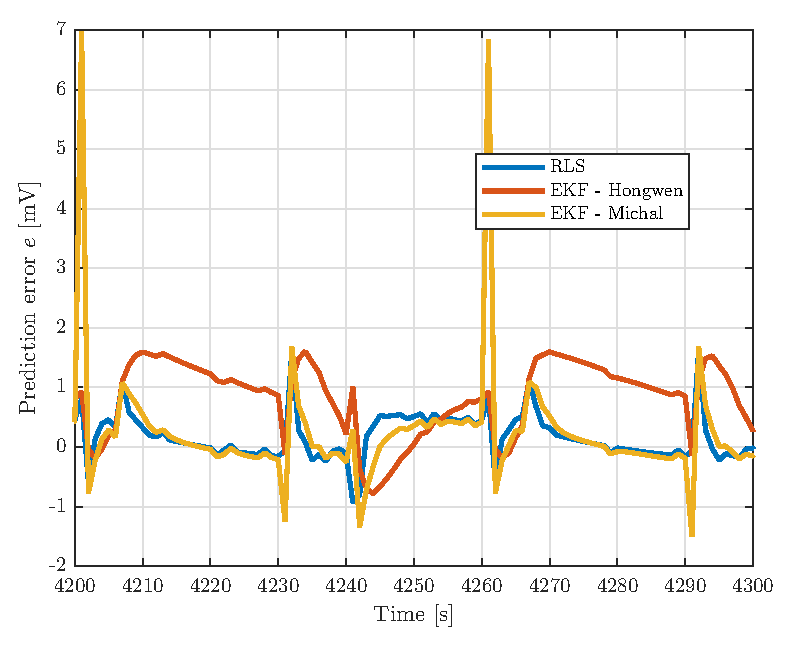
\includegraphics[width=\textwidth]{figures/10/voltages-pred-error.eps}
    \caption{Detail of one DDP period.}
    \label{fig:10-pred-error}
    \end{subfigure}
    
    \caption{Comparison of terminal voltages predicted by individual algorithms.}
    \label{fig:10-pred}
\end{figure}




\begin{figure}[hbp]
    \centering
\begin{subfigure}{0.49\textwidth}
    \centering
    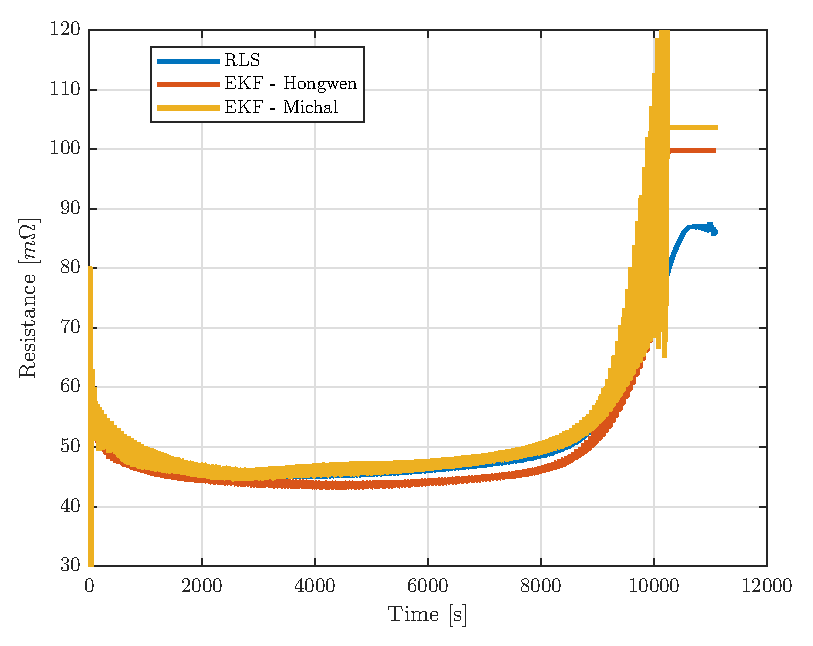
\includegraphics[width=\textwidth]{figures/10/est-R0.eps}
    \caption{Estimates of internal impedance $R_0$.}
    \label{fig:10-R0}
    \end{subfigure}
    \hfill
    \begin{subfigure}{0.49\textwidth}
    \centering
    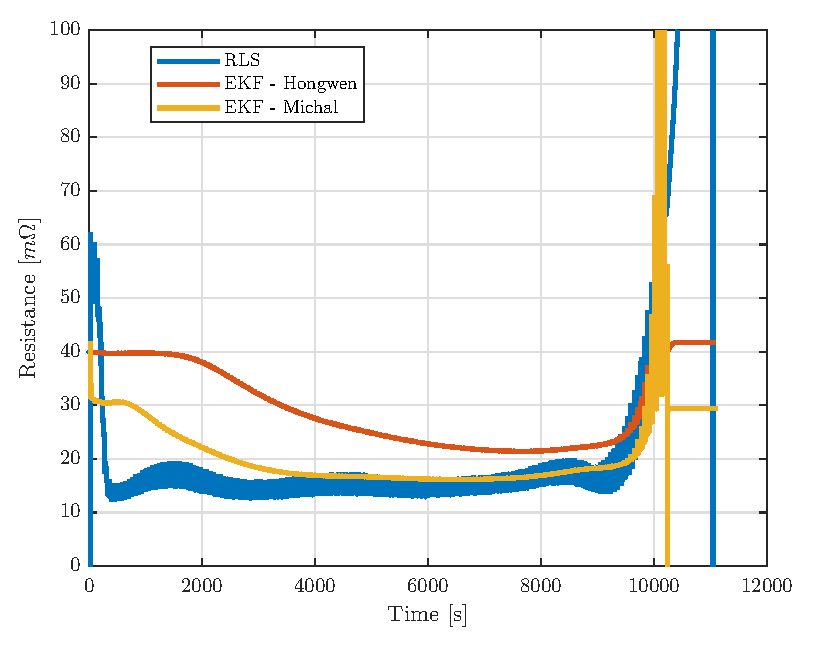
\includegraphics[width=\textwidth]{figures/10/est-R1.eps}
    \caption{Estimates of RC element resistance $R_1$.}
    \label{fig:10-R1}
    \end{subfigure}
    
    \caption{Estimates of resistive ECM parameters.}
    \label{fig:10-R}
\end{figure}

Estimates of both components of the ohmic (real) impedance $R_0$ and $R_1$ are shown in Fig. \ref{fig:10-R0} and Fig. \ref{fig:10-R1}, respectively. Estimates of $R_0$ yielded by various algorithms are quite similar and they demonstrate the expected (approximately) flat plateau roughly in the range of 80 \% to 20 \% of SoC with growing value towards extremes. On the other hand, estimates of $R_1$ shown in Fig. \ref{fig:10-R1} did not converge as satisfactorily with a significant discrepancy between both EKFs.

The estimated capacitance of the RC element shown in Fig. \ref{fig:10-C1} can be used to demonstrate an important difference between the RLS- and EKF-based parameter estimation. The EKF method allows the user to directly specify variance for individual physically meaningful parameters (albeit possibly inverted, such as $C_1^{-1}$). In contrast, the RLS works in terms of some artificial parameters $b_i$ and $a_i$, whose dependence on physically meaningful parameters is non-linear even for a 1 RC ECM and becomes increasingly more entangled with the growing number of parameters. Therefore, it is possible to get a smooth waveform for some given parameter (here $C_1$) with the EKF simply by reducing the parameter's variance. When estimating using RLS on the other hand, such fine control is very hard to do and the resulting estimate tends to be more noisy. A similar phenomenon can be observed in Fig. \ref{fig:10-R1}.

\begin{figure}[t]
\centering
\begin{minipage}{0.49\textwidth}
    \centering
    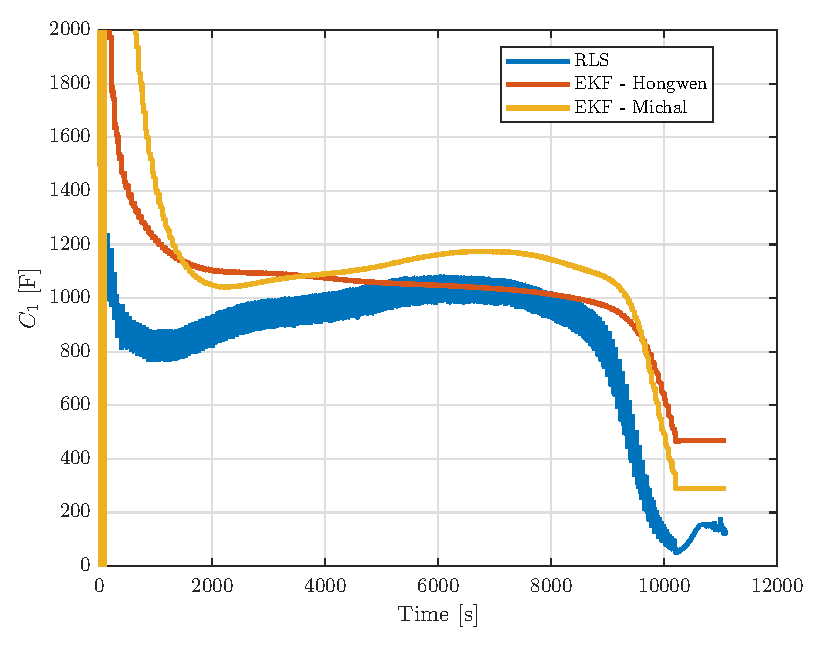
\includegraphics[width=\textwidth]{figures/10/est-C.eps}
    \caption{Estimates of RC element capacitance $C_1$.}
    \label{fig:10-C1}
\end{minipage}
\hfill
\begin{minipage}{0.49\textwidth}
    \centering
    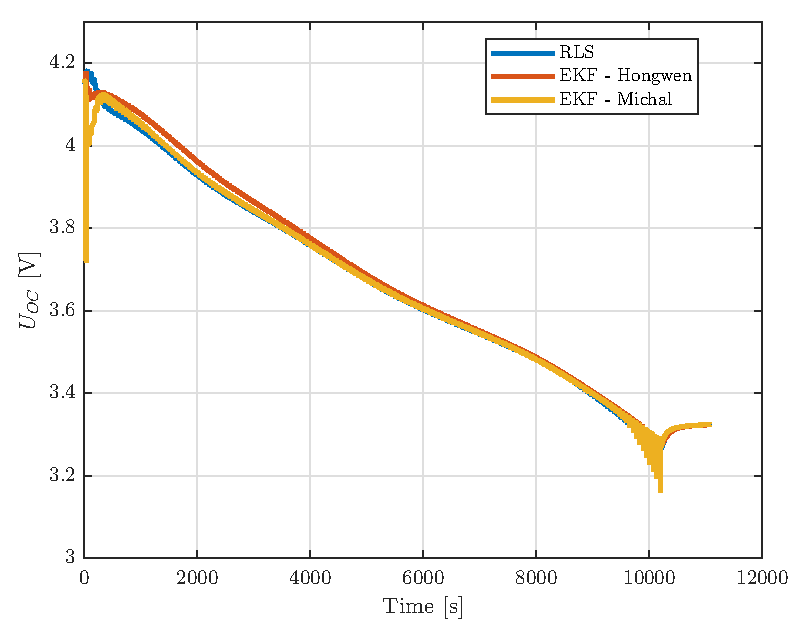
\includegraphics[width=\textwidth]{figures/10/est-OCV.eps}
    \caption{Estimates of the open circuit voltage $\OCV$.}
    \label{fig:10-OCV}
\end{minipage}
\end{figure}

All three methods estimate the $\OCV$ (shown in Fig. \ref{fig:10-OCV}) similarly well. The main difference from the implementation point of view is that the EKF method was far simpler to set up and debug owing to the tight bound of individual states to underlying physics. In contrast, the RLS method uses artificial (physically meaningless) parameters whose values must be post-processed to obtain any physically useful information. Typos such as an incorrect sign in some of the RLS expressions may cause a lot of headaches. Nevertheless, it is computationally less demanding than the EKF estimation and the forgetting factor $\lambda$ allows an intuitive configuration of the steady-state covariance matrix.

It is still unknown to me why the authors of \cite{hongwen} decided to use an unnecessarily complicated state space model for the parameter estimation task. Despite my best efforts in hyperparameter tuning (especially tuning the process noise covariance matrices $Q$), the simpler state-space model Michal achieved more credible results (closer matching the RLS estimates that I see as the best available reference in the absence of some ground truth parameter values) while being easier to debug and implement.

